\documentclass{article}
\usepackage[utf8]{inputenc}
\usepackage[margin=1in]{geometry}
\usepackage{nomencl}
\usepackage{standalone}
\usepackage{tikz}
\usetikzlibrary{shapes,trees,arrows}
\usepackage{multicol}
\usepackage{amsmath}


\title{Orifice Configuration Determination}
\author{Derek Bean}
\date{\today}

\bibliographystyle{ieeetr}
%%%%%%%%%%%%%%%%%%%%%%%%%%%%%%%%%%%%%%%%%%%%%%%%%%%%%%%%%%%%%%%%%%%%%%%%%%%%%%%%%%%%%%%%%%%%%%%%%%%%%%%%%%%%%
\usepackage{listings}
\usepackage{color}
\usepackage{courier}

%New colors defined below
\definecolor{codegreen}{rgb}{0,0.6,0}
\definecolor{codegray}{rgb}{0.5,0.5,0.5}
\definecolor{codepurple}{rgb}{0.58,0,0.82}
\definecolor{backcolour}{rgb}{0.95,0.95,0.92}

%Code listing style named "mystyle"
\lstdefinestyle{mystyle}{
  backgroundcolor=\color{backcolour},   commentstyle=\color{codegreen},
  keywordstyle=\color{magenta},
  numberstyle=\scriptsize\color{codegray},
  stringstyle=\color{codepurple},
  basicstyle=\small\ttfamily,
  breakatwhitespace=false,         
  breaklines=true,                 
  captionpos=b,                    
  keepspaces=true,                 
  numbers=left,                    
  numbersep=5pt,                  
  showspaces=false,                
  showstringspaces=false,
  showtabs=false,                  
  tabsize=2
}

\lstset{style=mystyle}
\usepackage{float}
    \restylefloat{table}
 \makenomenclature   
 
\newcommand{\dps }{ A k C_{d} \frac{\sqrt{\frac{2}{k+1}^{\frac{k+1}{k-1}}}}{\sqrt{\frac{kRT}{MW}}}}
\newcommand{\das}{P_o k C_{d} \frac{\sqrt{\frac{2}{k+1}^{\frac{k+1}{k-1}}}}{\sqrt{\frac{kRT}{MW}}}}
\newcommand{\dts}{ \frac{ A P_o C_{d} k^2 R}{2MW}
\frac{ \sqrt{2^{\frac{k+1}{k-1}}\left(\frac{1}{k+1}\right)^{\frac{k+1}{k-1}}}}
{\left(\frac{kRT}{MW}\right)^{\frac{3}{2}}}}

%%%%%%%%%%%%%%%%%%%%%%%%%%%%%%%%%%%%%%%%%%%%%%%%%%%%%%%%%%%%%%%%%%%%%%%%%%%%%%%%%%%%%%%%%%%%%%%%%%%%%%%%%%%%%
\begin{document}
\maketitle
\printnomenclature
        \nomenclature{$\dot{m}$}{mass flow rate of fluid ($\frac{kg}{s}$)}
        \nomenclature{$P_o$}{Upstream pressure ($kPa$)}
        \nomenclature{k}{ratio of specific heats}
        \nomenclature{R}{gas constant ($\frac{kPa\cdot m^3}{kmol\cdot k}$)}
        \nomenclature{MW}{molecular weight ($\frac{kg}{kmol}$)}
        \nomenclature{T}{temperature (K)}
        \nomenclature{$C_{d}$}{Discharge coefficient}
The goal of this Python code is to take in operating parameters of the Pulse Detonation Engine (PDE) and output the desired orifice diameters and upstream pressures to be set before operation. The input and output parameters are as follows:
    \begin{figure}[h]
        \centering
        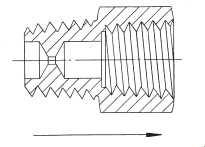
\includegraphics{Orifice_Image}
        \caption{Manufacturer drawing of orifice used}
        \label{fig:orifice}
    \end{figure}
    
\begin{multicols}{2}
    \subsection*{Inputs}
        \begin{itemize}
            \item Fuel
            \item Oxidizer
            \item Equivalence ratio
            \item Estimated gas temperature 
            \item Downstream pressure
            \item PDE length
            \item PDE inner diameter
            \item PDE operating frequency
            \item Maximum fuel pressure
            \item Maximum oxidizer pressure
            \item Minimum upstream pressure
            \item Possible orifice sizes
            
        \end{itemize}
\columnbreak
    \subsection*{Outputs}
        \begin{itemize}
            \item Fuel orifice size
            \item Fuel pressure setting 
            \item Oxidizer orifice size
            \item Oxidizer pressure setting 
        \end{itemize}
\end{multicols}
    
\section{Base Equations}
    Mass flow rate through an orifice. The equation used is eq. 3-24 from \textit{Rocket Propulsion Elements}~\cite{Sutton2001} with the discharge coefficient ($C_{d}$) added in. For this analysis $C_{d} = 0.99$ is used. 
        \[
        \dot{m} = AP_{o}k C_{d} \frac{\sqrt{\frac{2}{k+1}^{\frac{k+1}{k-1}}}}{\sqrt{\frac{kRT}{MW}}} \tag{Sutton 3-24}
        \]
    Since the unknowns in this equation are the area and upstream pressure of the orifice the mass flow rate equation can be rearranged, resulting in.
        \[
           AP_{o} = \frac{ \dot{m}\sqrt{\frac{kRT}{MW}}}{C_{d} k \sqrt{\frac{2}{k+1}^{\frac{k+1}{k-1}}}} 
        \]
        For the case where the orifice is not choked the equation becomes:
        \begin{equation*}
           \dot{m} = \rho A_{o} C_{d} \sqrt{\frac{2\left( P_{u}-P_{d} \right) }{\rho \left[ 1-\left(\frac{A_{o}}{A_{t}}\right)^{2}\right]}}
        \end{equation*}
\section{Calculation logic}
    \begin{figure}[H]
            \begin{center}
                \includestandalone[width=0.75\textwidth]{Logic_flow}
            \end{center}
            \end{figure}
\section{Error Analysis}
    Note that this analysis does not take the error in the solenoid actuation into account which may introduce more error especially in the start-up and shutdown periods of the gas flows. \\
    \subsection{Error Tree}
    
            \begin{figure}[h]
            \begin{center}
            \includestandalone[width=0.5\textwidth]{Orifice_Error_Tree}
            \end{center}
            \end{figure}
        Where:
        {\renewcommand\labelitemi{}
            \begin{itemize}
                \item  $R_{D} = \pm 0.0005in$
                \item  $R_{P_{o}} = \pm 17.2369 kPa$
                \item  $R_{T} = 2.2 K$
                \item  $R_{k} = 0$
                \item  $R_{R} = 0$
                \item  $R_{MW} = 0$
                \item  $R_{C_{d}} = 0$
            
            \end{itemize}
        }
        \[
            R_A=\sqrt{\left(\frac{\partial A}{\partial D}\cdot R_{D}\right)^2}=\sqrt{\left(\frac{\pi}{4}\cdot0.0005\right)^2}=0.000393D
        \]
        \[
            R_{\dot{m}}=\sqrt{\left(\frac{\partial \dot{m}}{\partial P_{o}}\cdot R_{P_{o}}\right) ^2+\left(\frac{\partial \dot{m}}{\partial A}\cdot R_{A}\right) ^2+\left(\frac{\partial \dot{m}}{\partial P_T}\cdot R_{T}\right) ^2}
        \]
        and the partial derivatives:
        \[
            \frac{\partial \dot{m}}{\partial P_o} = \dps%A k \frac{\sqrt{\frac{2}{k+1}^{\frac{k+1}{k-1}}}}{\sqrt{\frac{kRT}{MW}}}
        \]
        \[
            \frac{\partial \dot{m}}{\partial A} = \das %P_o k \frac{\sqrt{\frac{2}{k+1}^{\frac{k+1}{k-1}}}}{\sqrt{\frac{kRT}{MW}}}
        \]
        \[
            \frac{\partial \dot{m}}{\partial T} = \dts%\frac{ A P_o k^2 R}{2MW}
        %\frac{ \sqrt{2^{\frac{k+1}{k-1}}\left(\frac{1}{k+1}\right)^{\frac{k+1}{k-1}}}}
        %{\left(\frac{kRT}{MW}\right)^{\frac{3}{2}}}
        \]
        Which results in: 
        
        \[
            R_{\dot{m}}=\left[\left(\dps\cdot R_{P_{o}}\right) ^2 + \left(\das \cdot R_A \right) ^2 +\left( \dts \cdot R_T \right) ^2 \right]^{\frac{1}{2}}
        \]
\section{Codes}
    \subsection{Main File}
        The most recent version of the main code is shown below
            \lstinputlisting[language=Python]{flowproject.py}
    \subsection{Functions}
         The most recent collection of the functions is shown below
            \lstinputlisting[language=Python]{flowprojectfunc.py}

\bibliography{mendeley}


\end{document}